\section{Diagramas de secuencia}

\begin{figure}[H]
	\centering
	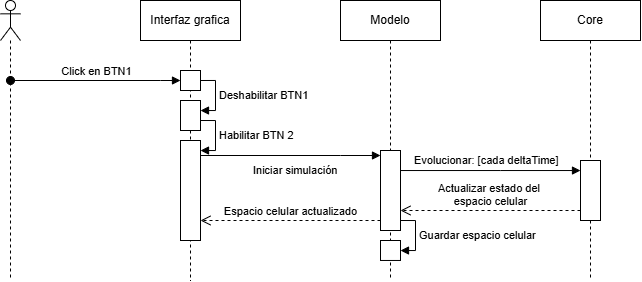
\includegraphics[width=0.9\linewidth]{img/UML_SD_UC01.png}
	\caption{Diagrama de secuencia: UC01 Iniciar simulación.}
	\label{fig:UML_SD_UC01}
\end{figure}

\begin{figure}[H]
	\centering
	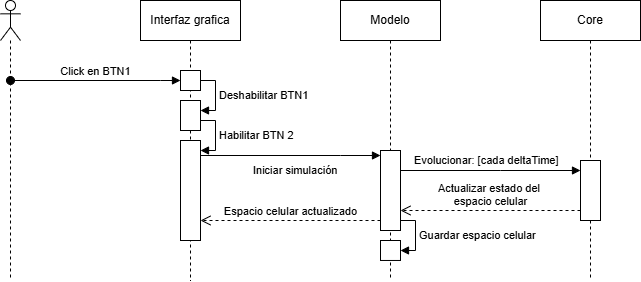
\includegraphics[width=0.9\linewidth]{img/UML_SD_UC02.png}
	\caption{Diagrama de secuencia: UC02 Pausar simulación.}
	\label{fig:UML_SD_UC02}
\end{figure}

\begin{figure}[H]
	\centering
	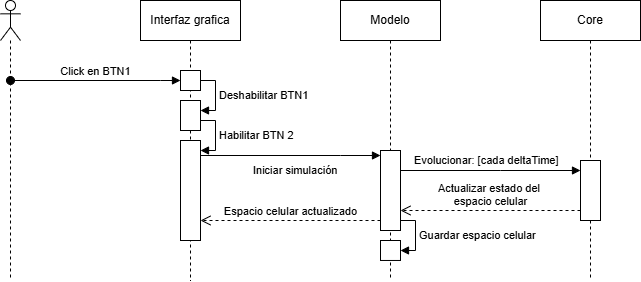
\includegraphics[width=0.9\linewidth]{img/UML_SD_UC05.png}
	\caption{Diagrama de secuencia: UC05 Simular un paso.}
	\label{fig:UML_SD_UC05}
\end{figure}

\begin{figure}[H]
	\centering
	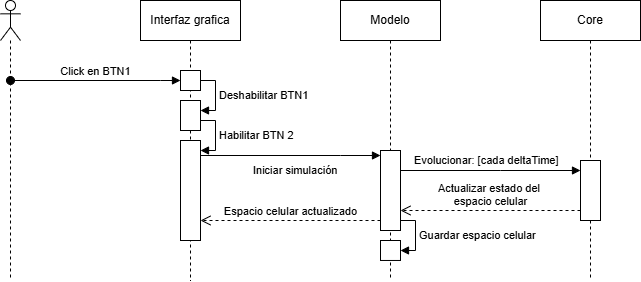
\includegraphics[width=0.9\linewidth]{img/UML_SD_UC06.png}
	\caption{Diagrama de secuencia: UC06 Retroceder un paso.}
	\label{fig:UML_SD_UC06}
\end{figure}

\begin{figure}[H]
	\centering
	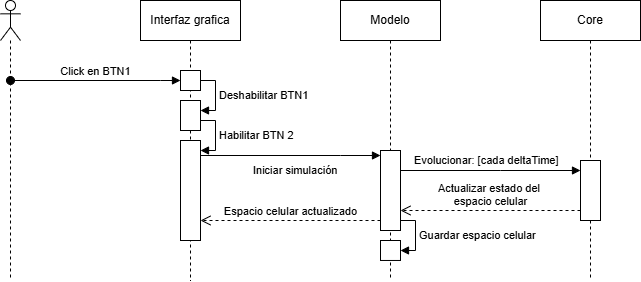
\includegraphics[width=0.9\linewidth]{img/UML_SD_UC08.png}
	\caption{Diagrama de secuencia: UC08 Definir vecindad.}
	\label{fig:UML_SD_UC08}
\end{figure}

\begin{figure}[H]
	\centering
	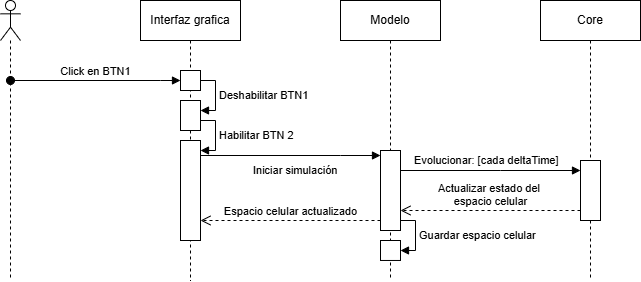
\includegraphics[width=0.9\linewidth]{img/UML_SD_UC11.png}
	\caption{Diagrama de secuencia: UC11 Definir numero de estados.}
	\label{fig:UML_SD_UC11}
\end{figure}

\begin{figure}[H]
	\centering
	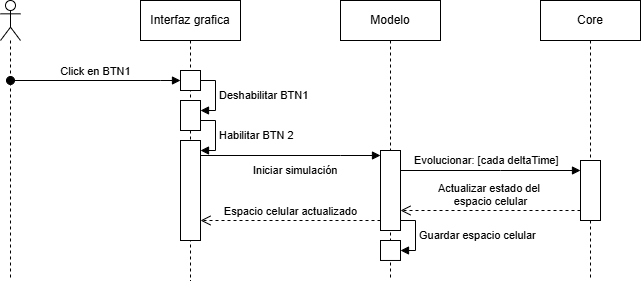
\includegraphics[width=0.9\linewidth]{img/UML_SD_UC12.png}
	\caption{Diagrama de secuencia: UC12 Definir función de transición.}
	\label{fig:UML_SD_UC12}
\end{figure}
